\documentclass[a4paper]{article}

\usepackage{amsmath}
\usepackage{amsthm}
\usepackage{amsfonts}
\usepackage[utf8]{inputenc}
\usepackage{csquotes}
\usepackage{listings}
\usepackage{graphicx}
\usepackage{ifthen}
\usepackage{xspace}
\usepackage{hyperref}
\usepackage{mathtools}
\usepackage{tikz}
\usepackage{caption}
\usepackage{subcaption}

\DeclarePairedDelimiter\ceil{\lceil}{\rceil}
\DeclarePairedDelimiter\floor{\lfloor}{\rfloor}

\newcommand{\pgap}{~\\\noindent}

\newcommand{\Fsh}{{F$\sharp$}\xspace}

\newcommand{\col}[2]{{\begin{pmatrix} #1 \\ #2 \end{pmatrix}}}
\newcommand{\mmod}{\text{ mod }}

\newtheorem{theorem}{Theorem}
\newtheorem{lemma}{Lemma}
\newtheorem{definition}{Definition}

\lstset{basicstyle=\small\ttfamily,frame=leftline,numbers=left,xleftmargin=0.7cm,basewidth=0.14cm}
\lstset{rangeprefix=(*, rangesuffix=*),includerangemarker=false}

\lstnewenvironment{Code}{}{}
\newcommand{\codeInput}[2][]{\ifthenelse{\equal{#1}{}}{\lstinputlisting[title=#2]{#2}}{\lstinputlisting[linerange=#1-end,title=#2\ -\ #1]{#2}}}
\newcommand{\code}{\lstinline}


\title{INTER 2}
\author{Carl Dybdahl, Patrick Hartvigsen, Emil Chr. Søderblom}
\usepackage[danish]{babel}

\begin{document}

\maketitle

\section*{Opgave 1: Billeje}
\begin{enumerate}
\item Billeje af en VW Golf(manuelt gear) med afhentning fra Ålborg Lufthavn den 23/02/2017 og aflevering den 23/02/2016 samme sted med udvidet selvrisikodækning koster 787.27 DKK.
\item Bilens dører får alvorlige skræmmer som koster 9000 DKK i reperationer. Men frygt ej! For du skal kun betale 5000 DKK ud af de 9000 DKK! Da du har en kaskoforsikring med en selvrisiko på 5000 DKK. \#PENGENESTOPPERALDRIG \#LEGALT \#ETISK \#HURTIGT
\end{enumerate}

\section*{Opgave 2: Heuristikker}

Mens vi løste opgaverne stødte vi på følgende eksempler på heuristikkerne:

\begin{figure}[!ht]
\centering
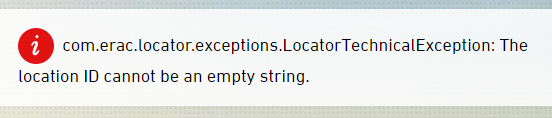
\includegraphics[width=0.5\textwidth]{error0.png}
\caption{Fejlen når vi prøver at gå videre til næste side efter at have valgt dato.}
\label{error-next}
\end{figure}

\begin{itemize}
\item Med det samme når vi går ind på hjemmesiden kører der en film i baggrunden. Vi føler at den er distraherende og bryder princip 8, simplificér.
\item Midt på forsiden er der en stor søgeboks, som effektivt fanger brugerens opmærksomhed og tilbyder at udføre hjemmesidens primære funktion. Søgeboksen sikrer at brugeren altid vælger en gyldig biludlejningssted, hvilket gør den til et positivt eksempel på princip 5, forebyg fejl.
\item Når vi skal til at søge efter Aalborg Lufthavn for at lave en bestilling, skriver vi "Aalborg Lu", hvilket leder til at hjemmesidens autofærdiggørelse viser en fejlmeddelelse. Fejlmeddelsen indeholder akavet sprog, f.eks. "Vi kunne ikke finde dette Aalborg Lu". Dette bryder princip 2, tal brugerens sprog.
\item Hjemmesiden har kun "Aalborg Airport" og ikke "Aalborg Lufthavn" i sin database. Dette er et problem for folk der bruger det danske navn for lufthavnen, og bryder princip 2, tal brugerens sprog.
\item Når man vælger data og tidspunkt guider hjemmesiden en med en kalenderwidget, som gør det nemmere at vælge dato en visse andre metoder. Alternativt kan man bare indtaste datoen direkte. Deres kalenderwidget er en god måde at følge princip 5, forebyg fejl, da den gør datoerne nemmere at visualisere.
\item Hvis man vælger at aflevere bilen klokken 22:00, vil dette være uden for Enterprise's åbningstid. Dette leder til at en besked bliver vist i bunden, men denne besked er blandet engelsk og dansk. Dette er uhensigtsmæssigt, og bryder princip 4, gør det ensartet.
\item På siden hvor vi skal vælge dato og klokkeslæt bliver vi også spurgt om en rabotkode eller et kunde-/virksomhedsnummer. Det er ikke tydeligt hvilken effekt det har eller hvordan man får fat i det, og der mangler en nem hjælpeknap til at vise det. Dette bryder princip 10, hjælp og dokumentation.
\item Da vi var ved at gå videre til næste trin fik vi en fejlmeddelelse, se figur \ref{error-next}. Denne fejlmeddelse hjælper ikke med at  løse problemet, og bryder dermed princip 9, hjælp når der er problemer.
\item Vi kan bruge menuen i bunden til at se vores tidligere indtastede data, hvilket er et positivt eksempel på princip 1, vis systemets tilstand.
\item Når hjemmesiden er i gang med at loade, bliver det gjort tydeligt ved at de fader siden og viser en ring af prikker. Dette er et godt eksempel på princip 1, vis systemets tilstand.
\item Hjemmesiden har en sprogvalgmulighed og en valutavalgmulighed, så brugeren selv kan vælge hvordan den er præsenteret. Dette er et positivt eksempel på princip 2, tal brugerens sprog.
\item Hvis vi ønsker at leje en bil i Farum er dette ikke muligt (se fejlmeddelelsen i figur \ref{error-farum}, sandsynligvis fordi Enterprise ikke har et biludlejningssted her. I dette tilfælde ville det være hensigtsmæssigt hvis hjemmesiden kunne vise nærmeste biludlejningssted, men det gør den ikke nemt. Dette bryder princip 6, støt hukommelse.
\end{itemize}

\begin{figure}[!ht]
\centering
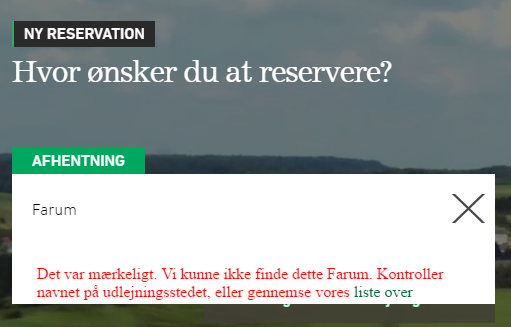
\includegraphics[width=0.5\textwidth]{error2.png}
\caption{Fejlen når en by ikke eksisterer.}
\label{error-farum}
\end{figure}


\end{document}	